\label{sec:intro}
\section{Analysis of Texture in Scene Images}

Texture refers to a surface characteristic and appearance of an object given by
its geometry, density and surface reflectance, and the stochastic variation of
these parameters.
It is a detailed pattern that is mapped into a multidimensional space.
It is an important cue in trying to achieve photo realistic
rendering of 3D models by adding surface details or color to an object or a
scene. Some of the natural scene textures are shown in Fig \ref{fig:natural}

3D Texture modeling is an important area in computer graphics as it results in realistic rendering
of natural material surfaces. The characterization of surface reflectance properties is important in
achieving photorealism. The appearance of a surface in different lighting and viewing direction/conditions 
is affected by its reflectance properties. 3D texture actually models the relation
between surface reflectance properties and illumination direction.

\begin{figure}[t]
\centering
\subfigure{

\includegraphics[height=1.5in,width=1.8in]{texture/1.eps}
}
\subfigure{

\includegraphics[height=1.5in,width=1.8in]{texture/2.eps}
}
\subfigure{

\includegraphics[height=1.5in,width=1.8in]{texture/3.eps}
}
\subfigure{

\includegraphics[height=1.5in,width=1.8in]{texture/7.eps}
}
\subfigure{

\includegraphics[height=1.5in,width=1.8in]{texture/8.eps}
}
\subfigure{

\includegraphics[height=1.5in,width=1.8in]{texture/9.eps}
}
\caption{Natural Scene Textures}
\label{fig:natural}
\end{figure}

\begin{figure}[hp]
\centering
\subfigure[]{
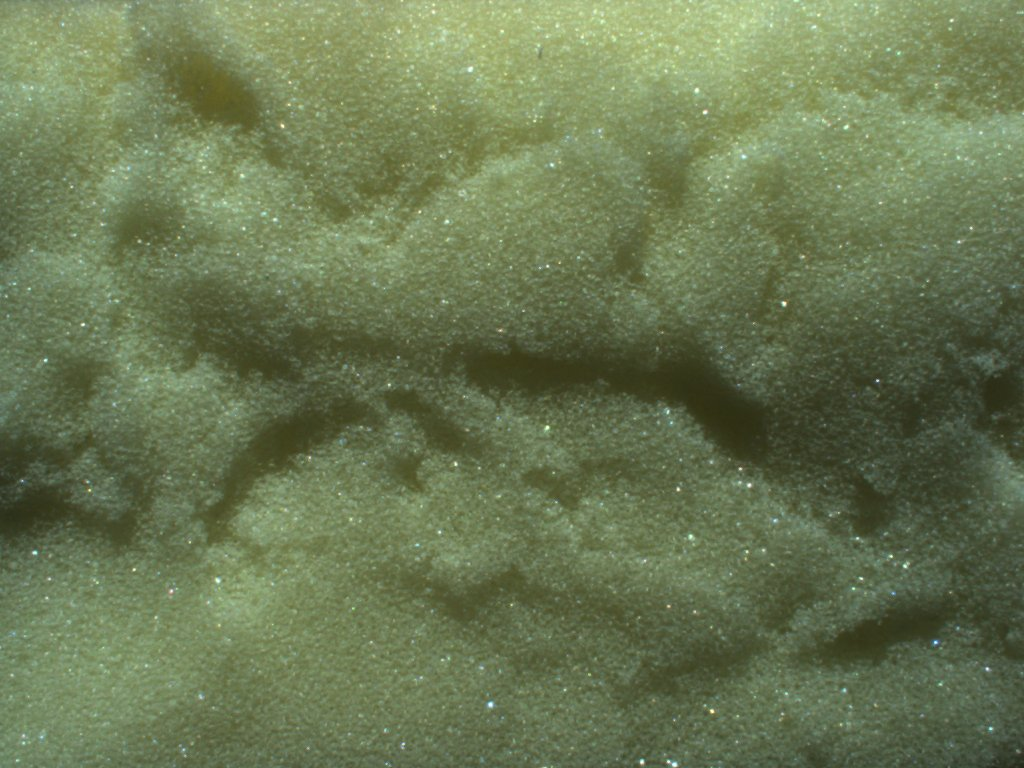
\includegraphics[scale=.18]{image_eps/orig_some/0.eps}
}
\subfigure[]{

\includegraphics[scale=.18]{image_eps/orig_some/9.eps}
}
\subfigure[]{

\includegraphics[scale=.18]{image_eps/orig_some/10.eps}
}
\subfigure[]{

\includegraphics[scale=.18]{image_eps/orig_some/26.eps}
}
\label{fig:3dtexture} 
\caption{Variation in appearance of the same surface
patch, when illuminated from different lighting directions}
\subfigure{
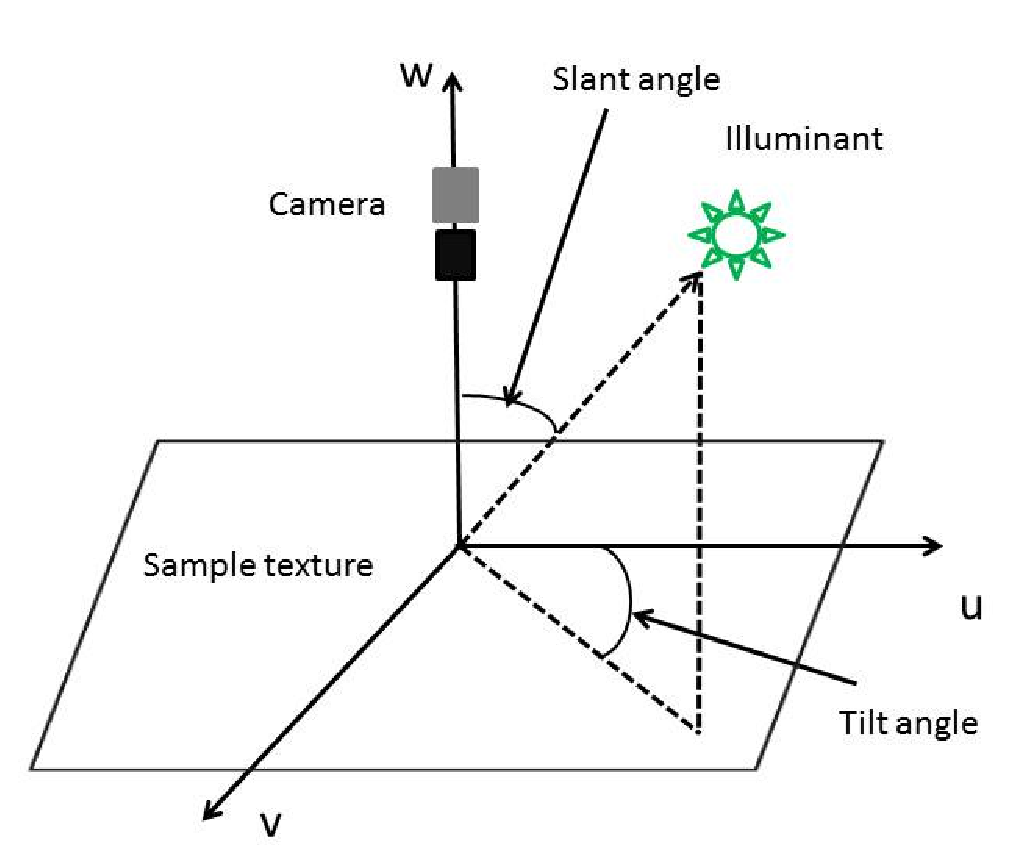
\includegraphics[scale=.58]{chap3/res_2/setup.eps}
}
\label{fig:setup}
\caption{Experimental setup}
\end{figure}

Mapping 2D textures or images is the most common method used, which is
efficient for most 3D models and scenes, especially where the lighting
conditions remain constant. They look best when the object is viewed in similar lighting conditions as
when the texture is captured. They appear flat and smooth.
In practice, the real world surfaces are
characterized by phenomena such as inter-reflection, self-shadowing, subsurface
scattering, specularity, etc. These properties interact with different lighting
directions and therefore the same surface appears different under
different lighting condition Fig 1.2. 2D texture fails to capture these complex reflectance properties of a 
surface and therefore a rendered surface looks highly unrealistic in case the lighting
conditions are changed. In order to produce a realistic rendering it is necessary to capture
and model the interaction of the material surface with different lighting
conditions. \cite{C1} investigates the problem of representation, recognition, synthesis of
natural materials and their rendering under arbitrary viewing/lighting conditions.

%%%%%%%%%%%%%%%%%FIGURE NO 1%%%%%%%%%%%%%%%

3D textures are a way to model this relation between surface reflectance
properties and illumination/viewing conditions.
The use of 3D texture modeling
results in enhanced realism of the scene. Reflectance texture maps are one of
the techniques that can be used to compactly represent the 3D textures. These
maps are generated using image re-lighting techniques \cite{C5,C4,C2} in which
multiple images are captured under different lighting conditions.

Image based modeling techniques \cite{C8,C6,C7} have emerged as
an effective approach for realistic rendering of 3D objects,
where multi-view geometry is utilized in directly synthesizing 
an unseen view of an object from nearby views without
explicit surface reconstruction. The traditional object models capture the shape information in the meshes,
while the reflectance and the surface properties are relegated in the textures. 3D models such as 
Polynomial Texture Maps (PTM) capture the 
surface properties more faithfully, including the effect of small scale height variation on the surface.

Polynomial Texture Maps \cite{C4} belong to the class of UTFs (Uni-directional Texture Function). It is a pixel
based technique that concisely models the surface reflectance properties using a
polynomial model for the reflectance, dependent on two angular parameters of the
lighting direction ($l_u$ and $l_v$). PTMs reconstruct the color of the surface under varying
lighting conditions and models real world phenomenon such as
self-shadowing, inter-reflection and sub-surface scattering. They thus introduce
enhanced photorealism in texture mapping.
Polynomial Texture Mapping is applied in a wide
range of archaeological contexts \cite{C14}. 
It also offers advantages over traditional raking
light photography for examining and
documenting the surface texture and
shape of paintings \cite{C13}.
Recently, PTMs have been used in cultural heritage field to document and virtually inspect 
several sets of small objects, such as cuneiform tablets and coins.

\subsection{Problem}
Texture mapping is an important area in computer graphics which adds realism to three dimensional 
models. 2D texture mapping fails to capture the surface variation and reflectance properties under
varying lighting and viewing direction. They appear good only when viewed from similar lighting
direction in which they were captured and fails to provide the information required for rendering other than the original
illumination condition. But 3D textures correctly models the relation between surface reflectance
properties and illumination conditions. The use of 3D texture modeling
results in enhanced realism of the scene.

But PTM technique causes overall smoothening of light which dampens the effect
of specularity and softens sharp shadows. The effect of point light source is
reduced and the appearance is always similar to a diffused light source.
Therefore we improve upon the PTM model 
to overcome the above limitations
and generate a complete 3D Texture model that can be evaluated at individual
pixels. We propose an approach to image-based lighting interpolation that is
based on estimates of geometry and shading from a set of input images.

\begin{figure*}[t]
\centering
%\subfigure[]{
\includegraphics[height=3.7in,width=6.2in]{sep_images/sep3.eps}
%\label{fig:subfig23} } \caption[] {Components of a sponge image: a) Original image, b) Direct c) Global
%component.} 

\caption{Component Based Modeling (CBM)}
\label{fig:CBM}
\end{figure*}

\subsection{Approach}
We capture multiple images of a static object with a static camera under varying
lighting conditions.
The scene is
illuminated using a high frequency checkerboard pattern using the projector. The
projector is moved to different lighting positions for the purpose of obtaining
images with different lighting directions. Experimental setup is shown in Figure 1.3.

When we separate the image of the texture into direct and the global part, we find
that the shadows and the specularity appear very strongly in the direct part,
as these are phenomena that involve light that reaches the surface point
directly from the light source. The fine details and the structure of the
material are very prominently visible in the direct part as they are observed
primarily through shadows. On changing the lighting direction, the change in the
luminance of the direct part is minimal as long as the surface point is directly
illuminated. The variations are introduced, primarily by self-shadowing and
specularity, both of which are abrupt changes as the lighting direction changes.
The global component contains the lighting of a surface point from other
parts in a scene, and hence it captures the overall illumination as well as
color variations of a surface with lighting direction. As the lighting direction
changes, the luminance value of the global part varies significantly.

Both direct and global components are separately analyzed to derive the
corresponding models and parameters. Given a new lighting direction, we use the
two models separately to generate the corresponding components, and combine them
to get the final image. Then for a new lighting direction, we can readily
interpolate both specular content as well as shadows.
The main contributions of this work are (1) Direct and Global modeling characterized by
shadows, specularity and luminance, 
(2) separate modeling and hence better capturing of shadows and specularity
and (3) per pixel function model to
achieve real-time rendering of enhanced 3D textures on GPU.
The method is shown to indeed
generate better results for non-observed lighting directions.
A complete flowchart of our model is shown in Fig \ref{fig:CBM}


\section{Analysis of Text in Scene Images}
\begin{figure*}[t]
\centering
\subfigure{
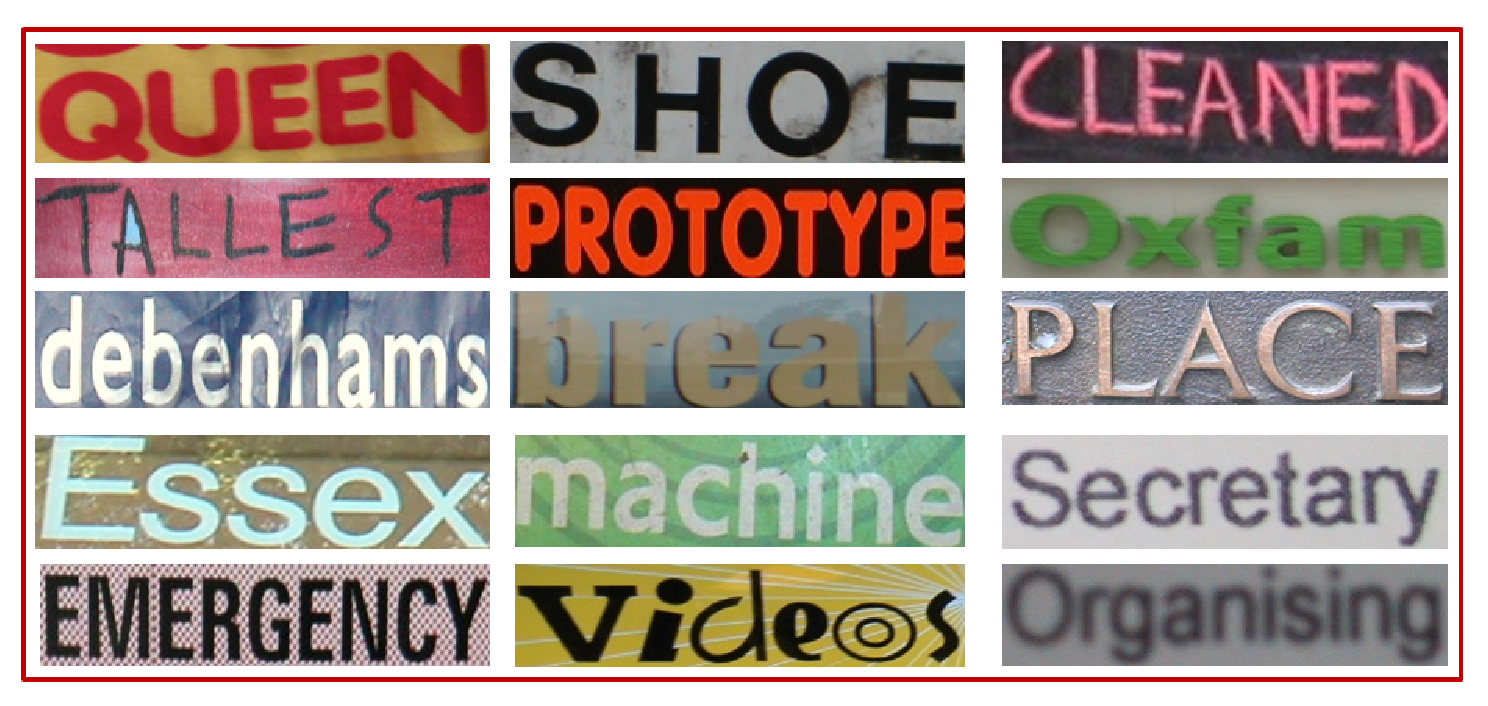
\includegraphics[height=3.6in,width=5.8in]{chap4/res_7/scene_text.eps}
}
\caption
{Natural Scene Text Images}
\label{fig:scenetext}
\end{figure*}
\begin{figure*}[t]
\centering
\subfigure{
\includegraphics[height=4.1in,width=5.5in]{chap4/res_7/text_chall.eps}
}
\caption
{Scene text images containing complex background}
\label{fig:textchallenge}
\end{figure*}

Scene text is textual content that is captured by a camera in an image.
Reading text captured in images provides valuable information and is
used in many content-based image
applications such as content based web image search,
information retrieval and mobile based text analysis
and recognition.

In the recent years, content-based image analysis techniques have received more attention with the 
advent of various digital image capture devices.
Applications of text localization
and recognition in real-world images ranges widely. It is used for indexing large image
databases by their textual content, sign recognition
for foreigners, automatic license plate recognition, assisting the elderly and visually
impaired in reading labels.

The images captured by these devices can vary dramatically depending on lighting conditions, reflections, 
shadows and specularity. Some natural scene text images are shown in Fig \ref{fig:scenetext}.
These images contain numerous degradations such as uneven lighting, complex background, multiple colors, blur etc.
We propose a method which removes reflections, shadows and specularity from natural scene text images and 
binarize the text from a single image.
Binarization method is one of the important pre-processing steps in document image analysis system. 
It directly affects the performance of the subsequent step which is text recognition.
Binarization of text can be defined as classifying individual pixels as foreground (text) or background. 

There are many algorithms that aim at extracting foreground text from background in images but thresholding remains one of
the oldest form that is used in many image processing applications. Many sophisticated approaches often have thresholding as a pre-processing step. 
It is often used to segment images consisting of bright objects against dark backgrounds or vice versa \cite{A1,A3,A4}.
It typically works well for images where the foreground and background are clearly defined.
For color thresholding images, most algorithms convert the 
RGB image into grayscale but here we will make use of the RGB channels as three different sources/components. 

Traditional thresholding based binarization can be grouped into two categories: the one which uses global
threshold for the given images like Otsu \cite{A2}, Kittler {\em et al}. 
\cite{A5} and the one with local thresholds like Sauvola \cite{A6},
Niblack \cite{A9}. In global thresholding methods \cite{A2,A7}, global thresholds are
used for all pixels in image. These methods are fast and robust as
they use a single threshold based on the global histogram of the gray-value pixels of the image.
But they are not suitable for complex
and degraded scene images. 
Also selecting the right threshold for the whole image is usually a challenge 
because it is difficult for the thresholding
algorithm to differentiate foreground text from complex background.

On the other hand, local or adaptive binarization \cite{A8} methods changes the threshold over the image according to local region properties.
Adaptive thresholding addresses variations in local intensities throughout the image.
In these methods, a per-pixel threshold is computed based on a local window around each pixel. 
Thus, different threshold values are used for different parts of the image. 
These methods are proposed to overcome global binarization drawbacks but they can be sensitive
to image artifacts found in natural scene text images like shadows, specularities and reflections.
On the other hand, we propose a method that removes shadows, specularity and reflections and thus produces a clean 
binary images even for the images with complex background.
\begin{figure*}[t]
\centering
\subfigure{
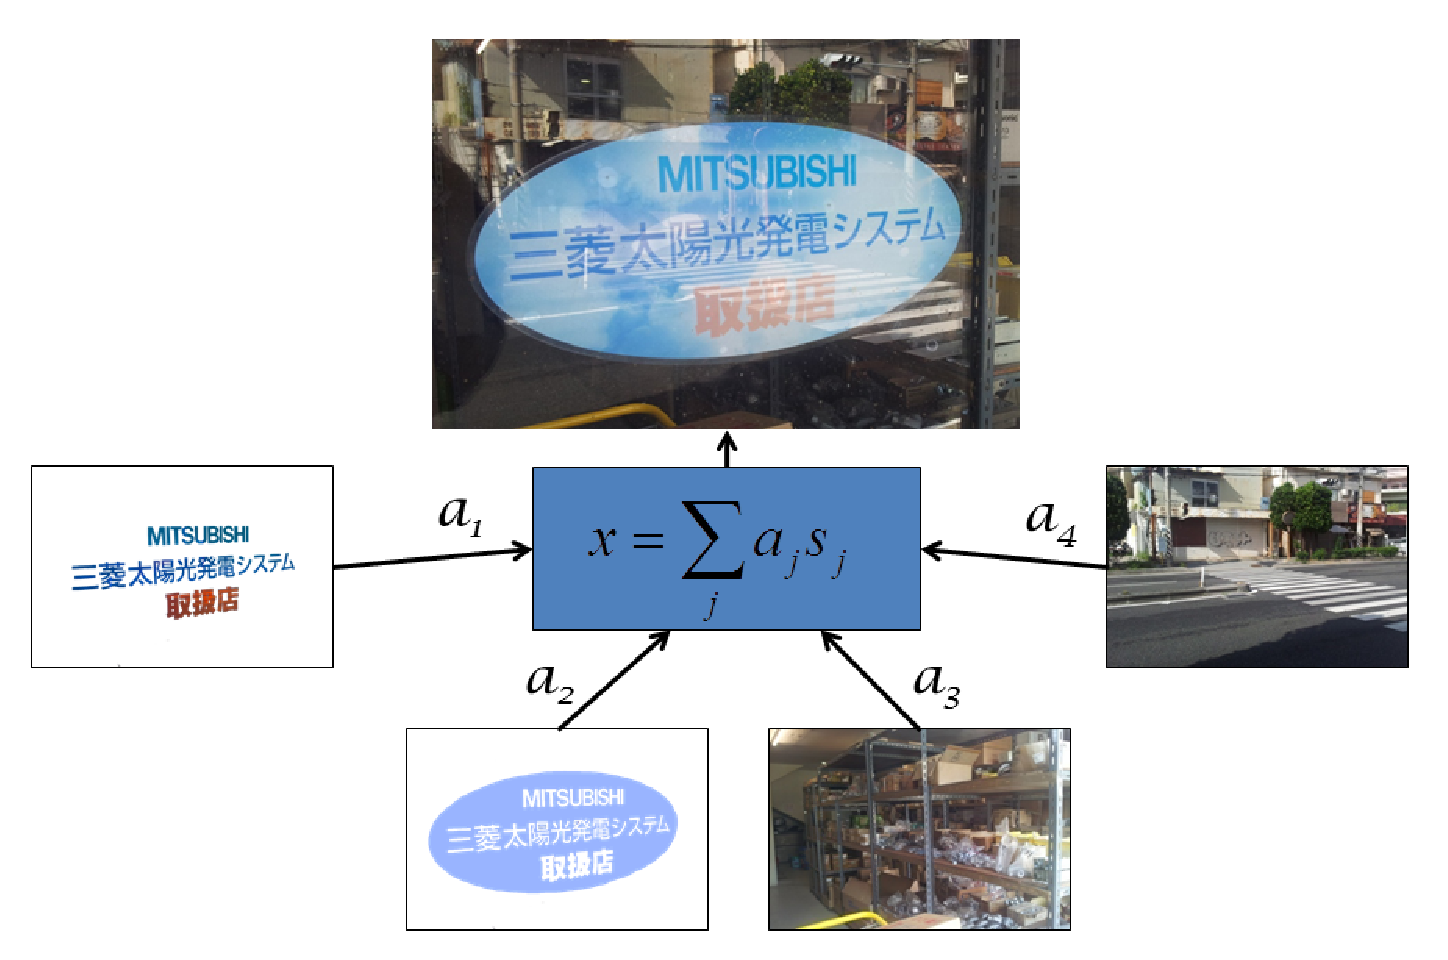
\includegraphics[height=3.8in,width=5.2in]{chap4/res_7/ica_model.eps}
}
\caption
{ICA model applied on images}
\label{fig:ICAmodel}
\end{figure*}
\subsection{Problem}
The primary issue related to segmenting text from scene images is the presence of complex/textured background. 
Some of the challenges are described below:
\begin{itemize}
\item \textbf{Noise:} Sensor noise in hand held camera devices is usually high.
\item \textbf{Viewing Angle:} While capturing images, the text and the camera device may not be parallel.
\item \textbf{Blur:} Some motion blur can
appear or be created by a moving object. Camera shake with hand-held shots can result in blurry images.
Camera not equipped with auto-focus also blurs the image.
\item \textbf{Resolution:} Depending on the capture device, resolutions of the images can vary from low to high.
\item \textbf{Non-planar surfaces:} Text written on non-planar objects like bottles can suffer from deformation.
\item \textbf{Low contrast:} It is difficult
to extract text when there is not much color difference between the foreground text and the background.
 \item \textbf{Lighting:}
Images containing uneven lighting, reflections, shadowing, highlights make colors of the text vary drastically and thus 
decreases analysis performance.
Both the physical environment and uneven response/artificial lighting from the camera devices are responsible for 
complexing the task of text extraction.
\end{itemize}
Some of the challenges that we encounter while segmenting natural scene text are shown in 
Fig \ref{fig:textchallenge}.

\subsection{Approach}
We apply an Independent Component Analysis (ICA) model on natural scene images.
It is one of the most important methods of blind source separation and has received  
attention in the field of signal processing, pattern recognition, data compression and image analyzing.
Using ICA,  we can extract the source signals from the 
observations based on the stochastic property of the input signals/images
even without any information of the original source signals.  
ICA method obtains features that present the data through a set of 
components that are statistically independent and characterizes the data 
in a natural way. 
ICA based decomposition enables us to separate text from complex backgrounds containing, reflections,
shadows and specularities. Fig \ref{fig:ICAmodel} shows the basic ICA model applied on images.
For binarization, we apply a global thresholding method on the independent components of the image
and that with maximum textual properties is used for extracting the foreground text. Binarization results show 
significant improvement in the extraction of text over other reported methods. 

\section{Outline}
In this chapter, we briefly analyzed textures and text in scene images. 
The rest of this thesis is organized as follows: 
We will survey techniques related to texture mapping and scene text understanding in Chapter 2. In Chapter 3
component based texture modeling will be discussed where we will show how each component is
modeled differently to achieve photorealism.
In Chapter 4, we will discuss component based text segmentation from natural scene images. Finally we 
conclude the thesis summarizing our main contributions and discuss future work in Chapter 5.

